\clearpage
\subsection{Summary} % (fold)
\label{sub:compilers_summary}

This chapter has introduced the concepts related to the tools you need to use to create programs. Computers can execute \textbf{machine code}, but this isn't very friendly for people to read or create. \textbf{Assembly code} provided the first layer of abstraction over machine code, giving symbolic names to the machine code instructions. This was a little easier to work with, but still required considerable work to create programs of even simple functionality. Most modern programs are written from \textbf{third generation languages} such as \textbf{C} and \textbf{Pascal}. With these languages the develop writes source code that is converted by a \textbf{compiler} into machine code.

\begin{figure}[h]
   \centering
   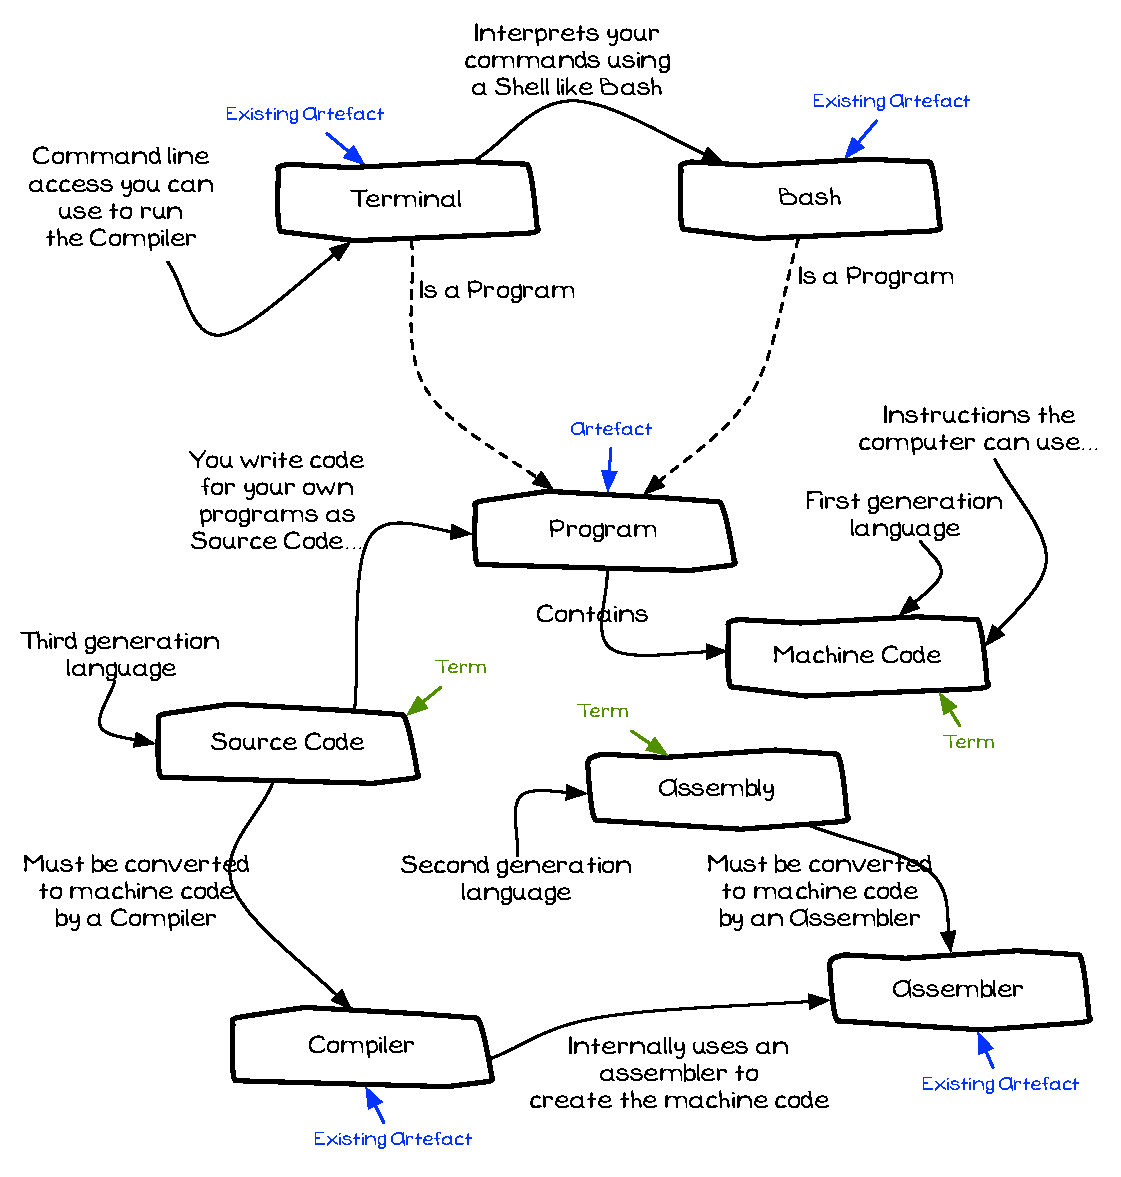
\includegraphics[width=0.9\textwidth]{./topics/programs-and-compilers/diagrams/Summary} 
   \caption{Overview of the topics covered in this chapter}
   \label{fig:compilers_summary}
\end{figure}

\mynote{
\begin{itemize}
  \item The \textbf{Terminal}, \textbf{Bash}, \textbf{Compiler}, and \textbf{Assembler} are all existing programs that you can use.
  \item \textbf{Source Code}, \textbf{Assembly Code}, and \textbf{Machine Code} are all terms for different ways that a program's instructions can be represented. Though Machine Code is the only form that can be executed directly by the machine.
\end{itemize}
}

% subsection summary (end)